% !TEX root = handbook-physics.tex
%!TEX TS-program = pdflatex
%!TEX encoding = UTF-8 Unicode


\chapter{Fundamentals of the Special Theory of Relativity}
\label{ch-05}
\zhtitle{狭义相对论基础}

\section{Postulates of the Special Theory of Relativity}
\label{sec-5.1}
\zhtitle{狭义相对论的公设}
\subsection{}\label{5.1.1} The \redem{special theory of relativity} (sometimes called the \redem{restricted relativity theory}) is the modern physical theory of space and time. The special relativity theory and quantum mechan­ics \ssect{38.1.1} serve as the theoretical basis for all modern physics and engineering (for example, nuclear physics and nuclear technology). The special relativity theory is often called \redem{relati­vistic theory}, and specific phenomena described by this theory
are called \redem{relativistic effects}. Relativistic effects are manifested, as a rule, at velocities of bodies close to that of light in free space ($c = \SI{3e8}{\meter\per\second}$) and called \redem{relativistic velocities}. Relati­vistic mechanics refers to the mechanics of motion at relativistic velocities and is based on the special theory of relativity.
\zhpar{\redem{狭义相对论}（有时也称为\redem{限制性相对论}）是关于空间和时间的现代物理理论。狭义相对论与量子力学\ssect{38.1.1}共同构成了全部现代物理学与工程技术（例如核物理和核技术）的理论基础。狭义相对论常被称为\redem{相对论}，该理论所描述的具体现象称为\redem{相对论效应}。相对论效应通常在物体速度接近真空中光速（$c = \SI{3e8}{\meter\per\second}$）时显现，这样的速度称为\redem{相对论速度}。相对论力学是研究相对论速度下运动的力学，它以狭义相对论为基础。}

As in classical Newtonian mechanics it is assumed in special relativity theory that time is uniform \ssect{3.4.2} and that space is homogeneous \ssect{2.7.1} and isotropic \ssect{4.4.1}.
\zhpar{与经典牛顿力学一样，狭义相对论假定时间是均匀的\ssect{3.4.2}，空间是均匀的\ssect{2.7.1}且各向同性\ssect{4.4.1}。}

\subsection{}\label{5.1.2} The special theory of relativity is based on two main principles accepted as the initial postulates.
\zhpar{狭义相对论建立在两条作为初始公设的主要原理之上。}

The \redem{first postulate} is a generalization of Galileo's mechanical principle of relativity \ssect{2.8.4} to cover any physical processes.
\zhpar{第一公设是将伽利略力学相对性原理\ssect{2.8.4}推广到任意物理过程。}

This postulate, called the \redem{principle of relativity}, or \redem{Einstein's relativity principle}, states: all physical phenomena proceed in the same way, under the same conditions, in all inertial frames of reference \ssect{2.1.2}. In other words, the principle of relativity contends that physical laws are independent (invariant) with respect to the chosen inertial frame of reference; equations expressing these laws have the same form in all inertial frames of reference. 
\zhpar{这一公设称为\redem{相对性原理}，或\redem{爱因斯坦相对性原理}，其内容是：在所有惯性参考系中，一切物理现象在相同条件下都以相同的方式进行。换言之，相对性原理认为物理定律相对于所选惯性参考系是独立的（不变的），表达这些定律的方程在所有惯性参考系中具有相同的形式。}

Consequently, it is impossible to ascertain, by means of any physical experiments whatsoever, conducted in a closed system of bodies \ssect{2.2.4}, whether the system is at rest or is travelling at uniform velocity in a straight line with respect to some inertial frame of reference. All inertial frames of reference are equally justified in physics. It is impossible, on the basis of physical experiments, to select from the host of inertial reference frames any ``preferred'' or ``absolute'' frame of reference possessing any qualitative distinctions from other inertial reference frames.
\zhpar{因此，借助在封闭物体系\ssect{2.2.4}中进行的任何物理实验，都无法确定该系统相对于某一惯性参考系是静止的，还是以恒定速度沿直线运动。所有惯性参考系在物理学中都具有同等的地位。仅凭物理实验，不可能从众多惯性参考系中挑选出任何在性质上不同于其他惯性参考系的“优越”或“绝对”参考系。}

\subsection{}\label{5.1.3} The \redem{second postulate} expresses the \redem{principle of the invariance of the velocity of light}: the velocity of light in free space is independent of the motion of the source of light. It is the same in all directions and in all inertial frames of reference, being one of the most basic physical constants. Experiments show that $c$, the velocity of light in free space, is the limiting velocity in nature. The velocity of any particles and bodies, as well as the velocity of propagation of any interactions or signals, cannot exceed $c$.
\zhpar{第二公设表述为\redem{光速不变原理}：真空中的光速与光源的运动无关。真空中光速在所有方向和所有惯性参考系中都相同，它是最基本的物理常量之一。实验表明，真空中的光速$c$是自然界中的极限速度。任何粒子和物体的速度，以及任何相互作用或信号的传播速度，都不能超过$c$。}

These specific laws governing the process of light propagation in free space enable this real physical process to be made use of in establishing a procedure for the \redem{chronometry of a frame of reference}, i.e. for the synchronization of clocks located at various points in space and travelling together with the frame of reference being considered \ssect{5.2.3}.
\zhpar{真空中光的传播所遵循的这些特定规律，使得人们能够利用这一真实的物理过程来建立\redem{参考系的计时方法}，即对位于空间不同点、并与所考虑的参考系一同运动的时钟进行同步\ssect{5.2.3}。}

\begin{marginfigure}%[!ht]
%\begin{wrapfigure}{r}{0.5\linewidth}
\centering
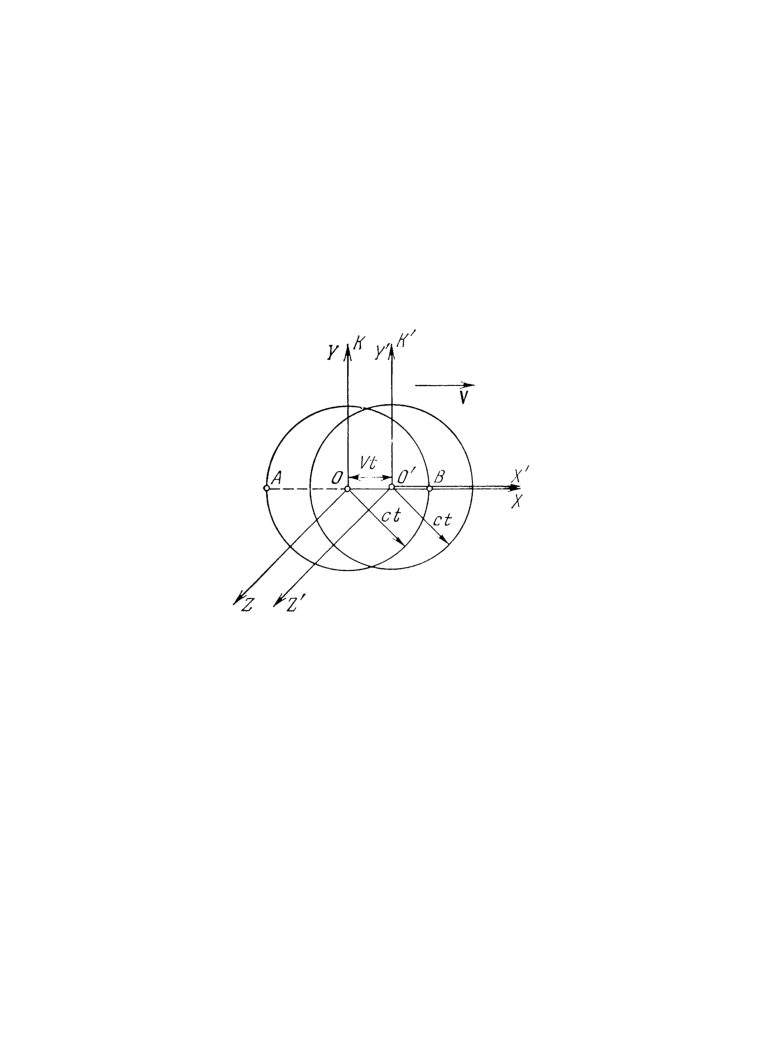
\includegraphics[width=0.8\textwidth]{figs/ch-05/fig-05-01.pdf}
%\input{figs/ch-03/fig-03-01}
%  \vspace{-13pt}
\sidecaption{Consequences of constancy of speed of light as a postulate in theory of relativity.\zhcap{光速不变性作为相对论公设的推论。}\label{fig-05-01}}
\end{marginfigure}

\subsection{}\label{5.1.4} The postulates of the special theory of relativity contra­dict the concepts of the properties of space and time that are accepted in classical mechanics and on which the Galilean transformations are based \ssect{2.8.1}. In particular, this refers to the contention, considered to be ``self-evident'' in Newtonian mechanics, that the passage of time is identical in all inertial frames of reference. From this it follows that the time interval between any two events is of an absolute nature. For instance, if two events occur simultaneously according to the clock in one inertial frame of reference, then, according to classical concepts, they also occur simultaneously according to the clock of any other inertial frame.
\zhpar{相对论公设与经典力学中关于空间和时间性质的概念相矛盾，而伽利略变换正是建立在这些概念之上的\ssect{2.8.1}。特别是，牛顿力学中被认为“不言自明”的观点——时间的流逝在所有惯性参考系中都是相同的——与之相矛盾。由此可知，任意两事件之间的时间间隔具有绝对的性质。例如，若两个事件按照某一惯性参考系中的时钟是同时发生的，那么按照经典概念，它们按照任何其他惯性参考系中的时钟也是同时发生的。}


The above-mentioned contradiction can be illustrated by the following example (\figr{fig-05-01}). We have two inertial frames of reference: fixed frame $K$ and frame $K'$ which travels along the $OX$ axis at constant velocity $V$. Assume that a flash of light is produced at point $O$ at the instant of the zero time reference in both frames $K$ and $K'$ $(t = t' = 0)$, when their origins $O$ and $O'$ of coordinates coincide. By the instant of time $t > 0$, light, propagating in free space at the velocity $c$, reaches points at the surface of a hollow sphere in the frame $K$. This sphere has its centre at point $O$ and its radius equals $ct$.
\zhpar{上述矛盾可以用下面的例子加以说明（\figr{fig-05-01}）。设有两个惯性参考系：静止参考系$K$，以及沿$OX$轴以恒定速度$V$运动的参考系$K'$。假定在两参考系的坐标原点$O$与$O'$重合、两参考系的零时刻$(t = t' = 0)$时，在点$O$处产生一次光闪。到时刻$t > 0$时，以速度$c$在真空中传播的光，在参考系$K$中到达以$O$为球心、半径为$ct$的空心球面上的各点。}

It can be assumed that in frame $K'$ the light flash occurred at the instant of time $t' = O$ at point $O'$. Hence, according to the postulates of the special theory of relativity, by the instant of time $t' = t$, light in frame $K'$ reaches points at the surface of a hollow sphere of the same radius $ct$ as in the frame $K$ but with its centre at point $O'$. At this instant, however, point $O'$ is not at point $O$, but at a distance of $Vt$ from this point. Hence, any attempt to combine the postulates of the special theory of relativity with classical conceptions of absolute time that elapses identically in all frames of reference leads to an absurdity: the light flash must \redem{simultaneously} reach points in space that belong to two different hollow spheres.
\zhpar{可以认为，在参考系$K'$中，光闪是在时刻$t' = O$于点$O'$处发生的。因此，根据狭义相对论的公设，到时刻$t' = t$时，参考系$K'$中的光到达以$O'$为球心、与参考系$K$中半径相同（均为$ct$）的空心球面上的各点。然而，此时点$O'$并不在点$O$处，而是与之相距$Vt$。因此，任何试图将狭义相对论的公设与“在所有参考系中相同地流逝”的经典绝对时间概念相结合的做法，都会导致荒谬的结论：光闪必须\redem{同时}到达属于两个不同空心球面的空间点。}

\section{Simultaneity of Events. Synchronization of Clocks}
\label{sec-5.2}
\zhtitle{事件的同时性。时钟的同步}

\subsection{}\label{5.2.1} The concept of the simultaneity of two or several events is extensively employed in making various physical measure­ments. For example, to determine the length $l$ of a rod, arranged along the axis $OX$ of reference frame $K$ and travelling with respect to this frame, it is necessary to note the values of the coordinates $x_{2}(t)$and $x_{1}(t)$ of the ends of the rod \redem{simultaneously}, i.e. at the same instant of time $t$. Then
\zhpar{在进行各种物理测量时，广泛运用了多个事件同时性的概念。例如，为了测定沿参考系$K$的$OX$轴放置、并相对于该参考系运动的杆的长度$l$，必须\redem{同时}记录杆两端的坐标$x_{2}(t)$和$x_{1}(t)$，即在同一时刻$t$进行记录。于是有}
\begin{equation*}%
l = \abs{\,x_{2}(t) - x_{1}(t)\,}.
\end{equation*}
The instant of time at which some event occurs (for instance, the launching or touchdown times of a spaceship) is determined by noting a clock's reading that is \redem{simultaneous} with the event being considered. This can be simply done by means of a clock located at the place where the event occurs. Hence, there should be many clocks located at various points in space in each frame of reference. Obviously, these clocks should be in agreement with one another, i.e. run \redem{synchronously}: their readings should be identical at each instant of time $t$.
\zhpar{某一事件发生的时刻（例如宇宙飞船发射或着陆的时刻），是通过读取与所考虑事件\redem{同时}的时钟读数来确定的。这可以通过位于事件发生地点的时钟简单地实现。因此，每个参考系中都应在空间各点设置许多时钟。显然，这些时钟应当彼此一致，即\redem{同步地}运行：在每一时刻$t$，它们的读数都应相同。}

\subsection{}\label{5.2.2} The synchronism of clocks located adjacently, i.e. at the same place in space, can be checked by the coincidence of their readings at each arbitrary instant of time. The synchronism of clocks that are separated in space at the points $A$ and $B$, distant from each other, could be checked in a similar manner if we had at our disposal standard time signals that could pro­pagate \redem{instantaneously} from $A$ to $B$. Experiments indicate, however, that this method is unfeasible because the velocity of any signal cannot exceed the velocity of light in free space.
\zhpar{位于同一地点（即空间中同一位置）相邻放置的时钟，其同步性可以通过它们在任意时刻的读数是否一致来检验。若手头有可以从$A$点\redem{瞬时地}传到$B$点的标准时间信号，那么对于相隔一定距离、分别位于点$A$和$B$的时钟，也可以用类似方法检验其同步性。然而，实验表明，这种方法是不可行的，因为任何信号的速度都不能超过真空中的光速。}

We can, however, proceed in the following manner. We can convey the clock from $B$ to $A$, check whether it is synchronous with the clock located at $A$, and then convey the clock carefully back to $B$. Then we can check whether the clock brought back to $B$ runs at the same rate as the clock left at $A$ by transmitting time signals from $A$ to $B$ after definite equal time intervals according to the clock at $A$. But it cannot be established by this procedure whether a shift in the zero time reference has occurred in the clock reading while it was being conveyed back to $B$, i.e. whether the clock brought back to $B$ is now fast or slow with respect to the clock at $A$ by a constant amount $\Delta t$. 
\zhpar{不过，我们可以按以下方式进行：将时钟从$B$点搬到$A$点，检查它与$A$点时钟是否同步，然后再小心地将时钟搬回$B$点。接着，按照$A$点时钟的读数，每隔确定的相等时间间隔从$A$点向$B$点发送时间信号，以检验搬回$B$点的时钟与留在$A$点的时钟走时是否相同。然而，用这种程序无法判断：在时钟被搬回$B$点的过程中，其读数的零点是否发生了偏移，即搬回$B$点的时钟相对于$A$点时钟是快了还是慢了一个恒定量$\Delta t$。}

\subsection{}\label{5.2.3} The problem of the synchronism of clocks separated in space at points $A$ and $B$ can be solved only by an unambiguous agreement (or definition) about when these clocks are to be regarded as synchronous. Einstein made use of a real physical process -- the propagation of light in free space -- as the basis for such a definition. He proceeded from the facts that the velocity of light in free space is the maximum possible velocity at which signals can be transmitted in nature and that it is identical in all directions and in all inertial frames of ref­erence.
\zhpar{位于空间不同点$A$和$B$的时钟之间的同步问题，只有通过明确约定（或定义）这些时钟在什么条件下被视为同步，才能得到解决。爱因斯坦以真实的物理过程——光在真空中的传播——作为这一定义的基础。他的出发点是：真空中的光速是自然界中信号能够传播的最大速度，并且光速在所有方向和所有惯性参考系中都相同。}

Assume that according to the clock at point $A$ the light signal is transmitted from this point at the instant of time $t_{1}$ and, after being reflected at point $B$, returns to $A$ at the instant of time $t_{3}$. Then, by definition, the clock at $B$ is in synchronism with that at $A$ if they run at the same rate and if, at the instant the light signal reaches $B$, the clock located there indicates the time $t_{2}= (t_{1}+ t_{3})/2$.
\zhpar{假设按照$A$点的时钟，光信号在时刻$t_{1}$从该点发出，经$B$点反射后，在时刻$t_{3}$返回$A$点。那么根据定义，若$B$点的时钟与$A$点的时钟走时速率相同，并且在光信号到达$B$点的瞬间，该处时钟指示的时刻为$t_{2}= (t_{1}+ t_{3})/2$，则称$B$点的时钟与$A$点的时钟同步。}

\subsection{}\label{5.2.4} According to the special theory of relativity, the passage of time may differ in different inertial frames of reference. Consequently, the time interval between any two definite events is relative: it can change in going over from one inertial reference frame to another. In particular, the simultaneity of two events occurring at different points separated in space is also relative. Events occurring simultaneously in one inertial frame of reference are not at all simultaneous in other inertial frames that are travelling with respect to the first frame. In some frames of reference one of these events occurs before the other event; in other frames it occurs after the other event. 
\zhpar{根据狭义相对论，时间的流逝在不同惯性参考系中可能不同。因此，任意两个确定事件之间的时间间隔是相对的：从一个惯性参考系过渡到另一个惯性参考系时，它可能发生变化。特别地，发生在空间不同点上的两个事件的同时性也是相对的。在一个惯性参考系中同时发生的事件，在相对于该参考系运动的其他惯性参考系中根本不是同时发生的。在某些参考系中，其中一个事件先于另一事件发生；而在另一些参考系中，它则后于另一事件发生。}

Thus, in the example illustrated in \figr{fig-05-01} \ssect{5.1.4}, the arrival of the light flash at points $A$ and $B$ are events that occur simultaneously in the fixed frame of reference $A$. In the travelling frame of reference $K'$ these events are not simultaneous. The light flash reaches $A$, receding from the light source $O'$, later than it reaches $B$, approaching the source $O'$.
\zhpar{因此，在\figr{fig-05-01} \ssect{5.1.4}所示的例子中，光闪到达点$A$和$B$是在静止参考系$K$中同时发生的两个事件。而在运动参考系$K'$中，这两个事件并不同时。光闪到达背离光源$O'$运动的点$A$，比到达接近光源$O'$的点$B$要晚。}

Events connected by a cause-and-effect relationship, i.e. by causality, cannot occur simultaneously in any frame of reference whatsoever, because any effect is due to some process initiated by the cause. At the same time, no process (physical, chemical, biological, etc.) can proceed instantaneously. Therefore, relativity does not contradict causality in any way. In any inertial frame of reference an event that is an effect always occurs later than the event causing this effect.
\zhpar{由因果关系（即因果性）联系起来的事件，在任何参考系中都不可能同时发生，因为任何结果都是由原因引起的某一过程所导致的。同时，任何过程（物理的、化学的、生物的等）都不可能瞬时完成。因此，相对论与因果性并无任何矛盾。在任何惯性参考系中，作为结果的事件总是晚于引起该结果的事件发生。}

\section{Lorentz's Transformations}
\label{sec-5.3}
\zhtitle{洛伦兹变换}

\subsection{}\label{5.3.1} It follows from the postulates of the special theory of relativity, as well as from the homogeneity \ssect{2.7.1} and isotropy \ssect{4.4.1} of space and the uniformity of time \ssect{3.4.2}, that the rela­tions between the coordinates and times of the same event in two inertial frames of reference are expressed by the \redem{Lorentz transformations}, rather than the Galilean transformations \ssect{2.8.1} used in classical (Newtonian) mechanics. According to the prin­ciple of relativity and the above-mentioned properties of the symmetry of space and time, the Lorentz transformations should he linear.
\zhpar{由狭义相对论的公设以及空间的均匀性和各向同性（\ssect{2.7.1}、\ssect{4.4.1}）与时间的均匀性（\ssect{3.4.2}）可知，同一事件在两个惯性参考系中的空间坐标与时间之间的关系，并非经典（牛顿）力学中所用的伽利略变换\ssect{2.8.1}，而是由\redem{洛伦兹变换}来表示的。根据相对性原理以及上述空间和时间的对称性质，洛伦兹变换应为线性变换。}

\subsection{}\label{5.3.2} The Lorentz transformations are in their simplest form if the like axes of the Cartesian coordinates of the fixed $(K)$ and moving $(K')$ inertial frames of reference are pairwise paral­lel to each other and if frame $K'$ travels with respect to frame $K$ at the constant velocity $V$ along axis $OX$ (\figr{fig-02-03}, see \ssect{2.8.1}). If, in addition, the zero time reference in both frames ($t = 0$ and $t' = 0$) is taken as the instant when the origins $O$ and $O'$ of coordinates of the two systems coincide, then the Lorentz transformations are of the form
\zhpar{当固定惯性参考系$K$与运动惯性参考系$K'$的同名坐标轴两两平行，且参考系$K'$相对于参考系$K$沿$OX$轴以恒定速度$V$运动时（见\figr{fig-02-03}，参见\ssect{2.8.1}），洛伦兹变换具有最简单的形式。若再取两参考系的零时刻（$t = 0$和$t' = 0$）为两坐标系的原点$O$与$O'$重合的瞬间，则洛伦兹变换具有下列形式：}

\begin{align*}%
x' & = \frac{x - Vt}{\sqrt{1 - \frac{V^{2}}{c^{2}}}}, & x  &= \frac{x' + Vt}{\sqrt{1 - \frac{V^{2}}{c^{2}}}}, \\
y & = y', &  y' & = y, \\
z & = z', &  z' & = z, \\
t & = \frac{t - Vx/c^{2}}{\sqrt{1 - \frac{V^{2}}{c^{2}}}}, &  t' &= \frac{t + Vx'/c^{2}}{\sqrt{1 - \frac{V^{2}}{c^{2}}}}.
\end{align*}
where $c$ is the velocity of light in free space.
\zhpar{式中$c$为真空中的光速。}


%\begin{center}
%\begin{tabular}{llll}
%$x' = \dfrac{x - Vt}{\sqrt{1 - \dfrac{V^{2}}{c^{2}}}}$ & $y = y'$ & $z  = z'$ & $t  = \dfrac{t - Vx/c^{2}}{\sqrt{1 - \dfrac{V^{2}}{c^{2}}}}$ \\
%\\
%$x  = \dfrac{x' + Vt}{\sqrt{1 - \dfrac{V^{2}}{c^{2}}}}$ & $y' = y$ & $z' = z$ 
% & $t' = \dfrac{t + Vx'/c^{2}}{\sqrt{1 - \dfrac{V^{2}}{c^{2}}}}$
%\end{tabular}
%\end{center}



\subsection{}\label{5.3.3} The Lorentz transformations show that not only the spatial coordinates of an event being considered are changed in going over from one inertial frame of reference to another, hut the corresponding instants of time as well. But a definite interrela­tion exists between the spatial coordinates $x'$, $y'$ and $z'$ of an event and the time instant $t'$ it occurs in an arbitrary inertial frame of reference $K'$. Hence, the quantity $\qty[(x')^{2}+ (y')^{2} + (z')^{2}- c^{2}(t')^{2}]$ is independent of the velocity $V$ of frame $K'$, i.e. it is identical in all inertial frames of reference:
\zhpar{洛伦兹变换表明，在从一个惯性参考系过渡到另一个惯性参考系时，不仅同一事件的空间坐标发生变化，相应的时刻也会改变。但是，事件的空间坐标$x'$、$y'$、$z'$与其在任意惯性参考系$K'$中发生的时刻$t'$之间存在确定的相互关系。因此，量$\qty[(x')^{2}+ (y')^{2} + (z')^{2}- c^{2}(t')^{2}]$与参考系$K'$的速度$V$无关，即它在所有惯性参考系中都具有相同的值：}
\begin{equation*}%
(x')^{2}+ (y')^{2} + (z')^{2}- c^{2}(t')^{2} = (x)^{2}+ (y)^{2} + (z)^{2}- c^{2}(t)^{2}.
\end{equation*}
The coordinate $x'$ and time $t'$ cannot be imaginary. It follows, therefore, from the Lorentz transformations that the velocity of relative motion of any two inertial frames of reference cannot exceed the velocity of light in free space $(V \leqslant c)$.
\zhpar{坐标$x'$和时间$t'$不可能是虚数。因此，由洛伦兹变换可知，任意两个惯性参考系之间的相对运动速度不能超过真空中的光速（$V \leqslant c$）。}

\subsection{}\label{5.3.4} According to Einstein's principle of relativity \ssect{5.1.2}, physical laws must comply with the condition of \redem{relativistic invariance (Lorentz invariance)}. This requirement implies that equations expressing physical laws retain their form in going over from one inertial frame of reference to another in accord­ance with the Lorentz transformations.
\zhpar{根据爱因斯坦相对性原理\ssect{5.1.2}，物理定律必须满足\redem{相对论不变性（洛伦兹不变性）}的条件。这一要求意味着：按照洛伦兹变换由一个惯性参考系过渡到另一个惯性参考系时，表达物理定律的方程保持其形式不变。}

The Lorentz transformations reduce to the Galilean transforma­tions \ssect{2.8.1} at $V \ll c$ or, more precisely, in the limit as $V/c \to 0$, i.e. as $c \to \infty$. In other words, the Galilean transforma­tions and classical (Newtonian) mechanics based on them are founded on the assumption of instantaneous propagation of interaction. Such an approximate approach is permissible only in considering the laws of mechanical motion of bodies at veloci­ties a great many times less than the velocity of light in free space.
\zhpar{当$V \ll c$时，或者更确切地说，当$V/c \to 0$即$c \to \infty$时，洛伦兹变换退化为伽利略变换\ssect{2.8.1}。换言之，伽利略变换以及以其为基础的经典（牛顿）力学，是建立在相互作用瞬时传播这一假定之上的。这种近似处理仅在研究速度远小于真空中光速的物体的力学运动规律时才是允许的。}

\begin{marginfigure}%[!ht]
%\begin{wrapfigure}{r}{0.5\linewidth}
\centering
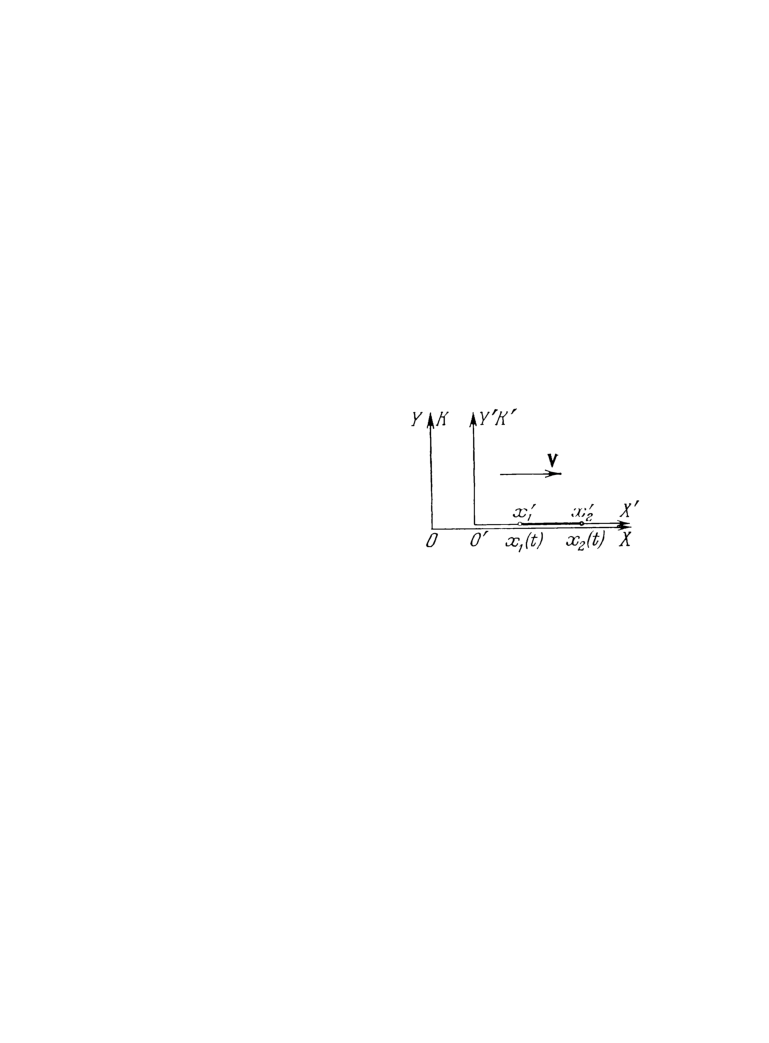
\includegraphics[width=0.8\textwidth,angle=-1]{figs/ch-05/fig-05-02.pdf}
%\input{figs/ch-03/fig-03-01}
%  \vspace{-13pt}
\sidecaption{Length contraction in relative motion.\zhcap{相对运动中的长度收缩。}\label{fig-05-02}}
\end{marginfigure}

\section[Relativity of Lengths and Time Intervals.]{Relativity of Lengths and Time Intervals. Time Interval Between Two Events}
\label{sec-5.4}
\zhtitle{长度和时间间隔的相对性。两事件之间的时间间隔}

\subsection{}\label{5.4.1} It follows from the Lorentz transformations \ssect{5.3.2} that the linear dimension of a body travelling with respect to an inertial frame of reference is reduced in the direction of motion. This change in the longitudinal size of a body in motionis called the \redem{Lorentz-FitzGerald contraction}. Assume $l_{0}$ to he the length of a rod at rest in reference frame $K'$. 
\zhpar{由洛伦兹变换\ssect{5.3.2}可知，相对于某一惯性参考系运动的物体，其线性尺寸在运动方向上会缩短。物体沿运动方向的纵向尺寸的这种变化称为\redem{洛伦兹-菲茨杰拉德收缩}。设$l_{0}$为相对于参考系$K'$静止的杆的长度。}

If the rod is located along axis $O'X'$ (\figr{fig-05-02}), then $l_{0}= x_{2}'-x_{1}'$, where $x_{2}'$ and $x_{1}'$ are the coordinates of the ends of the rod. The length $l$ of the same rod in reference frame $K$, with respect to which it travels along axis $OX$ at the velocity $V$, is equal to the difference in the coordinates of the ends of the rod, measured at the same instant of time $t$:
\zhpar{若杆沿$O'X'$轴放置（见\figr{fig-05-02}），则$l_{0}= x_{2}'-x_{1}'$，其中$x_{2}'$和$x_{1}'$为杆两端的坐标。杆在参考系$K$中（相对于该参考系沿$OX$轴以速度$V$运动）的长度$l$，等于同一时刻$t$测得的杆两端坐标之差：}
\begin{align*}%
l & =x_{2}(t) - x_{1}(t), \\
& =(x_{2}'-x_{1}')\sqrt{1 - \dfrac{V^{2}}{c^{2}}}, \\
& =l_{0}\sqrt{1 - \dfrac{V^{2}}{c^{2}}}.
\end{align*}
Transverse dimensions of a body are independent of its velocity and are identical in all inertial frames of reference:
\zhpar{物体的横向尺寸与其速度无关，在所有惯性参考系中都相同：}
\begin{equation*}%
y_{2} - y_{1} = y_{2}' - y_{1}',\,\,\textrm{and}\,\,z_{2} - z_{1} = z_{2}' - z_{1}'.
\end{equation*}
Thus, the linear dimensions of a body are relative. They are maximal in the inertial frame of reference with respect to which the body is at rest. These are
said to be the body's \redem{proper dimensions}.
\zhpar{因此，物体的线性尺寸是相对的。它们在相对于物体静止的惯性参考系中最大，这些尺寸称为物体的\redem{固有尺寸}。}


\subsection{}\label{5.4.2} The Lorentz-Fitzgerald contraction is a kinematic effect of the special theory of relativ­ity. It is not due to the effect of any kind of longitudinal forces compressing the body along its direction of motion. This contraction becomes appreciable only at velocities approaching
that of light in free space. It follows from the contraction formula that bodies cannot travel at velocities $V \geqslant c$ because at $V = c$ the longitudinal dimen­sion of the body (in the direction of motion) becomes zero, and at $V > c$ it would have to become imaginary.
\zhpar{洛伦兹-菲茨杰拉德收缩是狭义相对论的一种运动学效应，它并非由任何沿运动方向压缩物体的纵向力引起。这种收缩只有在速度接近真空中光速时才变得显著。由收缩公式可知，物体不能以$V \geqslant c$的速度运动，因为当$V = c$时，物体沿运动方向的纵向尺寸将变为零，而当$V > c$时它将变为虚数。}

\subsection{}\label{5.4.3} It is evident from the Lorentz transformations that in the theory of relativity we can specify a definite ``instant of time'' only with respect to a single definite inertial frame of reference. Thus, for instance, a single ``instant of time'' in ref­erence frame $K$ (a single definite value of time $t$ in this frame) corresponds to many values of time $t'$ in frame $K'$, depending upon the values of coordinate $x$:
\zhpar{由洛伦兹变换可以清楚地看出，在相对论中，只有相对于某一个确定的惯性参考系，才能规定一个确定的“时刻”。例如，参考系$K$中的一个“时刻”（即该参考系中时间$t$的一个确定值），对应于参考系$K'$中许多不同的时间值$t'$，具体取决于坐标$x$的数值：}
\begin{equation*}%
t' = \frac{t - Vx/c^{2}}{\sqrt{1 - \dfrac{V^{2}}{c^{2}}}}.
\end{equation*}
Likewise, a single ``instant of time'' in frame $K'$, i.e. a single definite value of time $t'$, corresponds to many values of time $t$ in frame $K$, depending upon the values of coordinate $x'$:
\zhpar{同样，参考系$K'$中的一个“时刻”（即时间$t'$的一个确定值），对应于参考系$K$中许多不同的时间值$t$，具体取决于坐标$x'$的数值：}
\begin{equation*}%
t = \frac{t' +  Vx'/c^{2}}{\sqrt{1 - \dfrac{V^{2}}{c^{2}}}}.
\end{equation*}


\subsection{}\label{5.4.4} Another important consequence of the Lorentz transformations is the relativity of the time interval between any two events (for example, the beginning and end of some process), i.e. the dependence of this time interval on the choice of the inertial frame of reference. Assume that two events, \hlblue{1} and \hlblue{2}, occur in the moving inertial frame of reference $K'$ at the same point $A$, fixed in frame $K'$ (i.e. $x_{2}'= x_{1}'$), at the instants of time $t_{1}'$ and $t_{2}'$. Thus, the time interval between the events is $\tau_{0}=  t_{2}'- t_{1}'$.
\zhpar{洛伦兹变换的另一个重要推论是：任意两个事件（例如某一过程的开始和结束）之间的时间间隔具有相对性，即该时间间隔依赖于所选的惯性参考系。设两个事件\hlblue{1}和\hlblue{2}在运动惯性参考系$K'$中于同一点$A$处发生（该点在$K'$中固定，即$x_{2}'= x_{1}'$），发生的时刻分别为$t_{1}'$和$t_{2}'$。于是，两事件之间的时间间隔为$\tau_{0}=  t_{2}'- t_{1}'$。}

With respect to fixed inertial frame of reference $K$, point $A$ travels with the same velocity $V$ as does frame $K'$. Hence in frame $K$ events \hlblue{1} and \hlblue{2} occur at different points in space, having the coordinates $x_{1}$ and $x_{2}$, and $x_{2} - x_{1} = V \tau$, where $\tau = t_{2}- t_{1}$ is the time interval between events \hlblue{1} and \hlblue{2} according to the clock in frame $K$. It follows from the Lorentz transformations that
\zhpar{相对于固定惯性参考系$K$，点$A$以与参考系$K'$相同的速度$V$运动。因此，在参考系$K$中，事件\hlblue{1}和\hlblue{2}发生在空间的不同点上，其坐标分别为$x_{1}$和$x_{2}$，且$x_{2} - x_{1} = V \tau$，其中$\tau = t_{2}- t_{1}$为参考系$K$中的时钟测得的事件\hlblue{1}与\hlblue{2}之间的时间间隔。由洛伦兹变换可得}
\begin{align*}%
\tau & = t_{2} - t_{1} =\frac{t_{2}'-t_{1}'}{\sqrt{1 - \dfrac{V^{2}}{c^{2}}}}, \\
& =\frac{\tau_{0}}{\sqrt{1 - \dfrac{V^{2}}{c^{2}}}}.
\end{align*}
Thus, the time interval between two events is minimal in the inertial frame of reference with respect to which both events occur at the same point. The time measured by a clock travel­ ling together with some object is said to be the \redem{proper time} of the object.
\zhpar{因此，两事件之间的时间间隔在如下惯性参考系中为最小：在该参考系中两事件发生在同一点上。与某一物体一同运动的时钟所测得的时间，称为该物体的\redem{固有时}。}

\subsection{}\label{5.4.5} The consequence of the Lorentz transformations that is dealt with in the preceding subsection is evidence of the existence of the relativistic effect of the slowing of time, called \redem{time dilation}, in a moving inertial frame of reference as compared to a fixed one. A clock travelling at the velocity $V$ with respect to a given inertial frame runs slower by a factor of $\sqrt{1 - V^{2}/c^{2}}$ than a fixed clock. Correspondingly, in agreement with the relativity principle, all physical processes in a moving frame of reference proceed at a slower rate than in a fixed frame.
\zhpar{上一小节中洛伦兹变换的推论，证明了存在一种相对论效应——时间变慢，称为\redem{时间延缓}：与静止参考系相比，运动惯性参考系中的时间变慢了。相对于某一惯性参考系以速度$V$运动的时钟，其走时速率为静止时钟的$\sqrt{1 - V^{2}/c^{2}}$倍，即比静止时钟走得慢。相应地，根据相对性原理，运动参考系中的所有物理过程都比静止参考系中的进行得慢。}

The time dilation effect becomes appreciable only at extremely high velocities $V$, close to that of light in free space. This effect has been demonstrated, for example, by experiments conducted with muons \ssect{43.3.3}. The muon is an unstable elementary particle. The mean proper lifetime of muons (according to a clock in the inertial frame of reference with respect to which they are at rest) $\tau_{0}= \SI{2.2e-6}{\second}$. Muons are created in the upper layers of title atmosphere by the action of primary cosmic rays, and they travel with respect to the earth at velocities $V$ close to $c$. If there was no relativistic effect of time dilation, a muon would be capable of travelling an average distance, with respect to an observer on the earth, of $\tau_{0}c = \SI{660}{\meter}$ through the at­mosphere. In other words, muons could not reach the earth's surface. Actually, they are registered by instruments installed at the surface of the earth, because the mean lifetime of a trav­elling muon, according to the clock of the observer on the earth, $\tau = \tau_{0}/\sqrt{1 - V^{2}/c^{2}} \gg \tau_{0}$, and the path travelled by a muon during this time, $\tau V \gg \SI{660}{\meter}$.
\zhpar{时间延缓效应只有在速度$V$极高、接近真空中光速时才变得显著。该效应已由\ssect{43.3.3}中的$\mu$子实验所证实。$\mu$子是一种不稳定的基本粒子，其平均固有寿命（按照与其静止的惯性参考系中的时钟计算）为$\tau_{0}= \SI{2.2e-6}{\second}$。$\mu$子在地球大气上层由初级宇宙射线的作用产生，它们相对于地球以接近$c$的速度$V$运动。如果不存在时间延缓的相对论效应，一个$\mu$子在大气中相对于地面观察者平均只能飞行$\tau_{0}c = \SI{660}{\meter}$的距离。换言之，$\mu$子将无法到达地球表面。实际上，它们被安装在地球表面的仪器探测到了，原因在于：按照地面观察者的时钟，运动$\mu$子的平均寿命为$\tau = \tau_{0}/\sqrt{1 - V^{2}/c^{2}} \gg \tau_{0}$，而在此期间$\mu$子所经过的路程为$\tau V \gg \SI{660}{\meter}$。}

\clearpage

\subsection{}\label{5.4.6} The relativistic effect of time dilation in a spaceship travelling with respect to the earth makes it feasible to under­ take space flights of almost unlimited length and journeys ``into the future''. According to the relativity principle, all processes in a spaceship, including the aging process of the astronauts, proceed in agreement with the same laws as on the earth. But in the spaceship time must be measured by a clock travelling together with it at the velocity $V$ with respect to the earth. 
\zhpar{运动飞船中的时间延缓相对论效应，使得进行长度几乎不受限制的太空飞行以及“进入未来”的旅行成为可能。根据相对性原理，飞船中的一切过程，包括宇航员的衰老过程，都遵循与地球上相同的规律。但在飞船中，时间必须用一个与飞船一同以相对于地球的速度$V$运动的时钟来测量。}

If $V$ is close to $c$ the clock in the ship runs considerably slower than earth clocks (at the space-launch complex), by a factor of $1/\sqrt{1 - V^{2}/c^{2}}$. For example, at $\beta = V/c = 0.99999$ the rates of the spaceship and earth clocks differ by a factor of 224. Consequently, in a time interval of $\tau_{0}= 10 \,\textrm{years}$ in such a spaceship, one can make a space flight taking $\tau = 2240\,\textrm{years}$ according to earth clocks, aging only 10 years during the flight. In this flight the spaceship can travel a tremendous distance from the earth: $l = V\tau = \beta c \tau = 2239.98 \,\textrm{light years}$\sidenote{A light year is the distance travelled by light in free space in one year: 1 light year = \SI{9.4605e15}{\metre}.}. The closer $V$ is to $c$, the greater the distance $l$ travelled by the spaceship with respect to the earth in the same interval $\tau_{0}$
of proper time in the spaceship, i.e. the longer the space flight that the astronauts can make during their lifetime.
\zhpar{若$V$接近$c$，飞船中的时钟将比地球上（发射场）的时钟走得慢得多，慢的倍数为$1/\sqrt{1 - V^{2}/c^{2}}$。例如，当$\beta = V/c = 0.99999$时，飞船时钟与地球时钟的走时速率相差224倍。因此，在飞船中经过$\tau_{0}= 10 \,\textrm{years}$的时间间隔内，按地球时钟计算，这次太空飞行将历时$\tau = 2240\,\textrm{years}$，而宇航员在飞行过程中只变老了10岁。在这次飞行中，飞船可以远离地球，距离达到$l = V\tau = \beta c \tau = 2239.98 \,\textrm{light years}$。$V$越接近$c$，在飞船固有时的同一时间间隔$\tau_{0}$内，飞船相对于地球所经过的距离$l$就越大，即宇航员在其一生中能够完成的太空飞行也就越长。}
\zhpar{注：光年是光在真空中一年内传播的距离：1光年 = \SI{9.4605e15}{\metre}。}

If an astronaut completes a space flight at a velocity $V$ close to $c$ by returning to the earth, he will find that people remaining on the earth (including his twin brother) has aged more than he has during the flight. If $V$ differs from $c$ by a sufficiently small amount, when $(1 - V^{2}/c^{2})^{-1/2} \gg 1$, the astronaut can, during the flight, outlive all his contemporaries and find him­ self, upon his return, among future generations.
\zhpar{如果宇航员以接近$c$的速度完成太空飞行后返回地球，他会发现留在地球上的人（包括他的孪生兄弟）比他老得多。若$V$与$c$的差值足够小，使得$(1 - V^{2}/c^{2})^{-1/2} \gg 1$，那么宇航员在飞行期间可以活过同时代的所有人，并在返回时发现自己置身于未来的世代之中。}

\subsection{}\label{5.4.7} It would seem, on the face of it, that, on the basis of the relativity principle, we should arrive at a conclusion exactly the opposite of that given in the preceding subsection. The clock on the earth, travelling at the velocity $-\vb{V}$ with respect to the spaceship, should run slower than the clock in the ship. There­fore, the time required for the flight should be longer for the astronaut, and not for the people left on the earth. Hence, the twin that made the flight should age more than his brother.
\zhpar{乍看起来，根据相对性原理，我们应当得出与上一小节完全相反的结论。相对于飞船以速度$-\vb{V}$运动的地球时钟，应当比飞船中的时钟走得慢。因此，飞行所需的时间对宇航员而言应更长，而不是对留在地球上的人而言更长。于是，进行飞行的那个孪生兄弟应当比他的兄弟衰老得更多。}

We have thus found that the difference between the readings of the clocks at the space-launch complex and in the ship is positive according to \ssect{5.4.6}, while, on the other hand, it is negative. This absurd result is called the \redem{clock}, or \redem{twin, paradox}. Actually, no clock paradox exists. It arose due to improper application of the relativity principle. This principle contends that not all frames of reference are equally justified, but only all \redem{inertial} frames of reference. But the frame of reference of the spaceship, in contrast to that of the earth, is not an inertial one all throughout the flight. During launching, turning around and in braking orbit when approaching the earth, the spaceship travels with acceleration (or deceleration). 
\zhpar{由\ssect{5.4.6}可知，发射场时钟与飞船中时钟的读数之差为正；另一方面，它却是负的。这一荒谬的结果称为\redem{钟佯谬}，或\redem{孪生子佯谬}。实际上，并不存在真正的钟佯谬，它是由于错误地应用相对性原理而产生的。该原理指出，并非所有参考系都具有同等的地位，只有所有\redem{惯性}参考系才具有同等地位。但在整个飞行过程中，飞船的参考系与地球参考系不同，并非始终是惯性系。在发射、掉头以及进入接近地球的制动轨道时，飞船都在作加速（或减速）运动。}

Consequently, the problem concerning the running of the clock at the launching complex which is always at rest with respect to a single inertial frame, and that of the clock in the spaceship, is, in principle, not a symmetrical one. Hence, the earth and ship frames of reference are not equally justified in the given problem. The reasoning in \ssect{5.4.6} is the correct one because it is based on the use of an inertial (the earth) frame of reference. Accord­ingly, the reasoning given in \ssect{5.4.7}, leading to the clock paradox, is incorrect. In the second case, the general theory of relativity should be applied, rather than the special theory. When this is done, it is found that, from the point of view of the astronaut as well, his clock runs slower than the clock at the launching complex.
\zhpar{因此，关于发射场上始终相对于同一个惯性参考系静止的时钟的走时问题，与飞船中时钟的走时问题，在原则上并不对称。所以在本问题中，地球参考系与飞船参考系并不具有同等的地位。\ssect{5.4.6}中的推理是正确的，因为它以惯性（地球）参考系为基础；相应地，\ssect{5.4.7}中导致钟佯谬的推理是不正确的。在后一种情形中，应当使用广义相对论，而非狭义相对论。这样处理后可以发现，从宇航员的角度看，他的时钟同样比发射场上的时钟走得慢。}

\subsection{}\label{5.4.8} The \redem{interval}, or \redem{space-time interval}, between two events, measured in the inertial frame of reference $K'$ is the quantity
\zhpar{在惯性参考系$K'$中测得的两事件之间的\redem{间隔}，或称\redem{时空间隔}，是如下的量：}
\begin{equation*}%
s_{12}' = \sqrt{c^{2}(t_{12}')^{2}-(l_{12}')^{2}},
\end{equation*}
where $t_{12}' = t_{2}' - t_{1}'$ is the time interval between the two events being considered (according to the clock in frame $K'$), and $l_{12}'= \sqrt{(x_{2}' -x_{1}')^{2}+(y_{2}' -y_{1}')^{2}+(z_{2}' -z_{1}')^{2}}$ is the distance between the points at which events \hlblue{1} and \hlblue{2} occur, also measured in frame of reference $K'$.
\zhpar{其中$t_{12}' = t_{2}' - t_{1}'$为两事件之间的时间间隔（按参考系$K'$中的时钟测量），$l_{12}'= \sqrt{(x_{2}' -x_{1}')^{2}+(y_{2}' -y_{1}')^{2}+(z_{2}' -z_{1}')^{2}}$为事件\hlblue{1}和\hlblue{2}发生地点之间的距离，同样在参考系$K'$中测量。}

It follows from the Lorentz transformations that the interval between two given events, \hlblue{1} and \hlblue{2}, is invariant with respect to the choice of the inertial frame of reference, i.e. it does not change in transferring from moving inertial frame $K'$ to fixed frame $K$:
\zhpar{由洛伦兹变换可知，两事件\hlblue{1}和\hlblue{2}之间的间隔相对于惯性参考系的选择是不变的，即在从运动惯性参考系$K'$变换到静止参考系$K$时，它并不改变：}
\begin{equation*}%
s_{12}' = s_{12} = \textrm{inv}, \,\,\textrm{where}\,\, s_{12} = \sqrt{c^{2}t_{12}^{2}-l_{12}^{2}}.
\end{equation*}
If $s_{12}^{2}> 0$, i.e. if $s_{12}$ is a real number, the interval $s_{12}$ is said to be \redem{timelike}.
\zhpar{若$s_{12}^{2}> 0$，即$s_{12}$为实数，则称间隔$s_{12}$为\redem{类时的}。}

The interval $s_{12}$ is said to be \redem{spacelike} if $s_{12}^{2} < 0$, i.e. $s_{12}$ is an imaginary number.
\zhpar{若$s_{12}^{2} < 0$，即$s_{12}$为虚数，则称间隔$s_{12}$为\redem{类空的}。}

\subsection{}\label{5.4.9} It follows from the invariance of the interval with respect to the choice of the inertial frame $K'$ that in all frames $K'$ the values of $t_{12}'$ and $l_{12}'$ for the giv­en two events, \hlred{1} and \hlred{2}, satis­fy the equation of a hyperbola:
\zhpar{由间隔相对于惯性参考系$K'$的选择的不变性可知，在所有参考系$K'$中，对于给定的两个事件\hlred{1}和\hlred{2}，$t_{12}'$与$l_{12}'$的值满足双曲线方程：}
\begin{equation*}%
c^{2}(t_{12}')^{2} - (l_{12}')^{2} = s_{12}^{2}.
\end{equation*}
If $s_{12}^{2} > 0$ the relation between $t_{12}'$ and $l_{12}'$ in various inertial frames of reference $K'$ travelling with respect to fixed frame $K$ at any possible velocities $(0 \geqslant V < c)$, can be represented graphically as the two branches
\hlred{I} and \hlred{II} of a hyperbola (\figr{fig-05-03}).
\zhpar{若$s_{12}^{2} > 0$，则在相对于静止参考系$K$以可能的任意速度$(0 \geqslant V < c)$运动的各参考系$K'$中，$t_{12}'$与$l_{12}'$之间的关系可以用双曲线的两支\hlred{I}和\hlred{II}直观地表示（见\figr{fig-05-03}）。}
\begin{marginfigure}%[!ht]
%\begin{wrapfigure}{r}{0.5\linewidth}
\centering
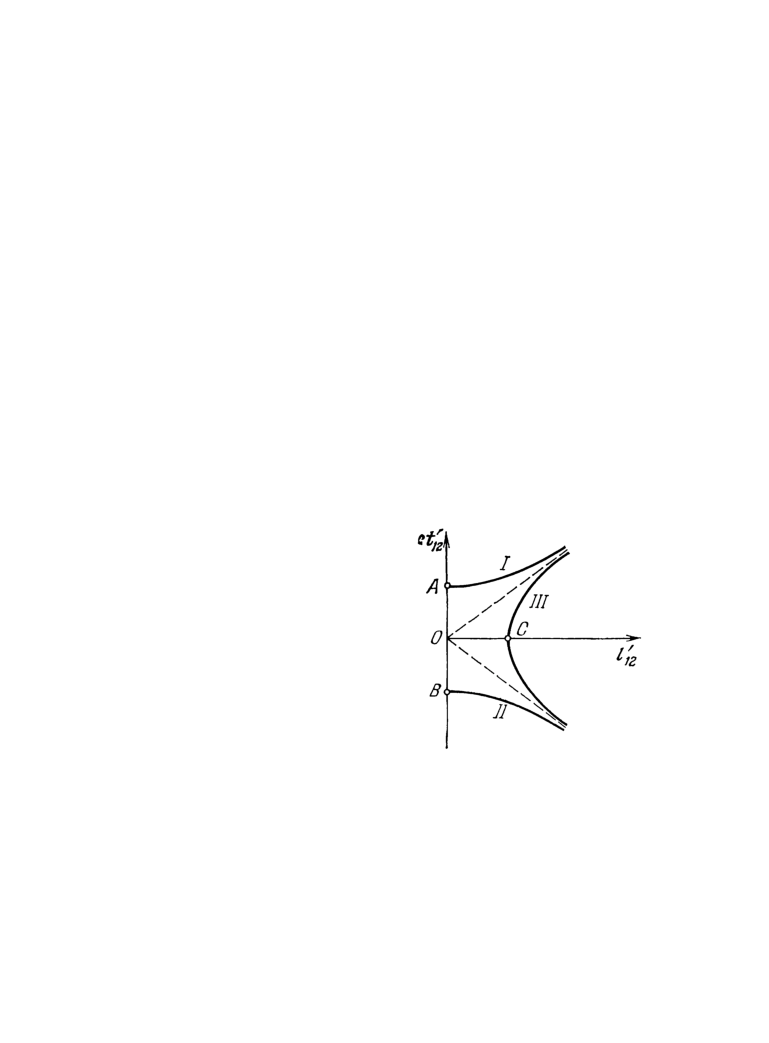
\includegraphics[width=0.8\textwidth]{figs/ch-05/fig-05-03.pdf}
%\input{figs/ch-03/fig-03-01}
%  \vspace{-13pt}
\caption{The invariance of interval between two inertial frames.\zhcap{两惯性参考系之间间隔的不变性。}\label{fig-05-03}}
\end{marginfigure}
Consequently, the sign of the time interval between events \hlblue{1} and \hlblue{2}, related by a timelike interval, is absolute. It is indepen­dent of the choice of the frame of reference: in all frames $K'$ the second event always occurs either after the first, i.e. $t_{12}' > 0$ (branch \hlred{I}) or always before the first, i.e. $t_{12}' < 0$ (branch \hlred{II}). The distance $l_{12}'$ is relative; an inertial frame $K'$ can be chosen in which $l_{12}' = 0$, i.e. events \hlblue{1} and \hlblue{2} occur at the same place (points $A$ and $B$ on the branches \hlred{I} and \hlred{II} of the hyperbola).
\zhpar{因此，由类时间隔联系的两事件\hlblue{1}和\hlblue{2}之间时间间隔的符号是绝对的，与参考系的选择无关：在所有参考系$K'$中，第二个事件总是发生在第一个事件之后，即$t_{12}' > 0$（分支\hlred{I}），或者总是发生在第一个事件之前，即$t_{12}' < 0$（分支\hlred{II}）。而距离$l_{12}'$是相对的：可以选取某一惯性参考系$K'$，使得$l_{12}' = 0$，即事件\hlblue{1}和\hlblue{2}发生在同一地点（即双曲线分支\hlred{I}和\hlred{II}上的点$A$和$B$）。}

Two events related by causality should always correspond to a timelike interval or, in any case, one equal to zero $(s_{12} = 0)$. This is due to the fact that the signal by means of which event \hlblue{1} (the cause) leads to event \hlblue{2} (the effect) cannot be propagated in space at a velocity exceeding that of light in free space:
\zhpar{因果关系相联系的两个事件，其间隔应当始终为类时的，或者至少等于零$(s_{12} = 0)$。这是因为，事件\hlblue{1}（原因）通过某种信号导致事件\hlblue{2}（结果），而该信号在空间中的传播速度不能超过真空中的光速：}
\begin{equation*}%
l_{12}' \leqslant c (t_{2}' - t_{1}').
\end{equation*}


\subsection{}\label{5.4.10} In the case of events related by a spacelike interval $(s_{12}^{2}< 0)$, the sign of $t_{12}'$ is relative: $t_{12}' > 0$ (upper part of hyper­ bola \hlred{III} in \figr{fig-05-03}) in certain inertial frames $K'$ whereas in others $t_{12}' < 0$ (lower part of hyperbola \hlred{III}). Point $C$ corres­ponds to the frame $K'$ in which $t_{12}' = 0$, i.e. events \hlblue{1} and \hlblue{2} occur simultaneously.
\zhpar{对于由类空间隔联系的两事件$(s_{12}^{2}< 0)$，$t_{12}'$的符号是相对的：在某些惯性参考系$K'$中$t_{12}' > 0$（双曲线\hlred{III}的上支，见\figr{fig-05-03}），而在另一些惯性参考系中$t_{12}' < 0$（双曲线\hlred{III}的下支）。点$C$对应于参考系$K'$，在该参考系中$t_{12}' = 0$，即事件\hlblue{1}和\hlblue{2}同时发生。}


\section[Transformation of Velocities and Accelerations]{Transformation of Velocities and Accelerations in Relativistic Kinematics}
\label{sec-5.5}
\zhtitle{相对论运动学中速度和加速度的变换}

\subsection{}\label{5.5.1} The velocities $\vb{v}$ and $\vb{v}'$ of a particle in two inertial frames of reference $K$ and $K'$ are
\zhpar{粒子在两个惯性参考系$K$和$K'$中的速度$\vb{v}$与$\vb{v}'$分别为}
\begin{align*}%
\vb{v} & = \dv{\vb{r}}{t} = v_{x}\vu{i}+ \vb{v}_{y}\vu{j}+ \vb{v}_{z}\vu{k}, \,\, \textrm{and},\\
\vb{v}'& =  \dv{\vb{r}'}{t'} = v_{x'}'\vu{i}'+ \vb{v}_{y'}'\vu{j}'+ \vb{v}_{z'}'\vu{k}',
\end{align*}
where $\vb{r} = x\vu{i}+ y\vu{j}+ z\vu{k}$ and $\vb{r}'= x'\vu{i}'+ y'\vu{j}'+ z'\vu{k}'$ are the radius vectors of the particle in frames $K$ and $K'$. The projections of velocities $\vb{v}$ and $\vb{v}'$ on the axes of Cartesian coordinates of frames $K$ and $K'$ are:
\zhpar{式中，$\vb{r} = x\vu{i}+ y\vu{j}+ z\vu{k}$与$\vb{r}'= x'\vu{i}'+ y'\vu{j}'+ z'\vu{k}'$分别为粒子在参考系$K$和$K'$中的位矢。粒子速度$\vb{v}$与$\vb{v}'$在参考系$K$和$K'$的笛卡儿坐标轴上的投影为：}
\begin{align*}%
v_{x} & = \dv{x}{t},& v_{y} &= \dv{y}{t},& v_{z} & = \dv{z}{t}, \\
v_{x'}' & = \dv{x'}{t'}, & v_{y'}' &= \dv{y'}{t'},& v_{z'}' &= \dv{z'}{t'}.
\end{align*}
If the like axes of the Cartesian coordinates of frames $K'$ and $K$ are pairwise parallel, and frame $K'$ travels with respect to frame $K$ at the constant velocity $V$ along axis $OX$ (\figr{fig-02-03}, see \ssect{2.8.1}) and, in addition, if at the zero time references in frames $K$ and $K'$ ($t = 0$ and $t' =0$), the origins $O$ and $O'$ of coordinates of these frames coincide, the Lorentz transforma­tions in the form given in \ssect{5.3.2} are valid. It follows from these transformations that the relations between the projections of the velocities of the particle on the axes of the Cartesian coordi­nates of frames $K$ and $K'$ are of the form:
\zhpar{若参考系$K'$与$K$的同名笛卡儿坐标轴两两平行，参考系$K'$相对于参考系$K$沿$OX$轴以恒定速度$V$运动（见\figr{fig-02-03}，参见\ssect{2.8.1}），并且在两参考系的零时刻（$t = 0$和$t' =0$）两坐标系的原点$O$与$O'$重合，则\ssect{5.3.2}中给出形式的洛伦兹变换成立。由这些变换可得，粒子速度在参考系$K$和$K'$的笛卡儿坐标轴上的投影之间的关系为：}
\begin{align*}%
v_{x} & = \dv{x}{t},& v_{y} &= \dv{y}{t},& v_{z} & = \dv{z}{t}, \\
v_{x'}' & = \dv{x'}{t'}, & v_{y'}' &= \dv{y'}{t'},& v_{z'}' &= \dv{z'}{t'}.
\end{align*}
These equations express the \redem{law of the composition of velocities in relativistic kinematics}. In the limit as $c \to \infty$ these equations lead to the ordinary law for the composition of velocities in classical mechanics \ssect{2.8.2}:\begin{align*}%
v_{x'}' & = v_{x} - V,\quad v_{y'}' = v_{y},\quad v_{z'}' = v_{z},\,\, \textrm{and},\\
\vb{v}' &= \vb{v} - \vb{V}.
\end{align*}
\zhpar{这些方程表达了\redem{相对论运动学中的速度合成定律}。当$c \to \infty$时，这些方程退化为经典力学中的通常速度合成法则\ssect{2.8.2}。}

\subsection{}\label{5.5.2} The relations between the squares of the magnitudes of vectors $\vb{v}$ and $\vb{v}'$ are
\zhpar{矢量$\vb{v}$与$\vb{v}'$的大小平方之间的关系为}
\begin{align*}%
v^{2} & = c^{2}\left[1 - \frac{\qty[1 - (v'/c)^{2}]\left(1-(V/c)^{2}\right)}{\left(1+Vv_{x'}'/c^{2}\right)^{2}} \right],\\
(v')^{2} & = c^{2}\left[1 - \frac{\qty[1 - (v/c)^{2}]\left(1-(V/c)^{2}\right)}{\left(1 - Vv_{x}/c^{2}\right)^{2}} \right].
\end{align*}
In particular, if $v' = c$, then $v = c$ and vice versa. Hence, if the velocity of a particle with respect to some inertial frame of reference is equal to the velocity of light in free space, then it must have the same magnitude with respect to any other inertial frame regardless of the velocity of relative motion of these two frames. In other words, the sum of two velocities, of which one is equal to $c$, is always equal to $c$. This law, detect­ed in the motion of such elementary particles as photons \ssect{37.1.4} and the neutrino (\tabl{tab-43.1}), demonstrates the limiting nature of the velocity of light in free space \ssect{5.1.3}.
\zhpar{特别地，若$v' = c$，则$v = c$，反之亦然。因此，若粒子相对于某一惯性参考系的速度等于真空中的光速，则它相对于任何其他惯性参考系的速度大小也必然等于$c$，而与两参考系之间相对运动的速度无关。换言之，若两个速度之一等于$c$，则二者之和始终等于$c$。这一规律在光子\ssect{37.1.4}和中微子（\tabl{tab-43.1}）等基本粒子的运动中已被观测到，它表明真空中的光速具有极限性质\ssect{5.1.3}。}
%(Table 43.1)
\subsection{}\label{5.5.3} It is evident from the equations in the preceding subsection that a particle, travelling with respect to some inertial frame of reference at a velocity less than $c$, has a velocity with respect to any other inertial frame that is also less than $c$ (for instance, if $v < c$, then $v' < c$, and vice versa). From this it follows, among other things, that no matter how close to $c$ the velocities of two particles are, their relative velocity is always less than $c$. Assume, for example, that two particles are travelling toward each other along the axis $OX$ of frame $K$ at the respective velocities: $\vb{v}_{1}= 0.8c\,\vu{i}$ and $\vb{v}_{2}= -0.8c\,\vu{i}$. The velocity $\vb{u}_{21}$ of the second particle with respect to the first is not equal, as is assumed in classical mechanics, to the vector difference $\vb{v}_{2} - \vb{v}_{1} = -1.6c\,\vu{i}$ if only because the magnitude of this velocity exceeds $c$. The required velocity is equal to the velocity of the second particle with respect to inertial frame $K'$, travelling together with the first particle ($\vb{V}=0.8c\,\vu{i}$), i.e. $\vb{u}_{21}= \vb{v}_{2}'$. It follows from the equation in \ssect{5.5.1} that
\zhpar{由上一小节的方程可知，相对于某一惯性参考系以小于$c$的速度运动的粒子，相对于任何其他惯性参考系的速度也小于$c$（例如，若$v < c$，则$v' < c$，反之亦然）。由此可知，无论两粒子的速度多么接近$c$，它们之间的相对速度总是小于$c$。例如，设两粒子沿参考系$K$的$OX$轴相向运动，速度分别为$\vb{v}_{1}= 0.8c\,\vu{i}$和$\vb{v}_{2}= -0.8c\,\vu{i}$。第二个粒子相对于第一个粒子的速度$\vb{u}_{21}$，并不等于经典力学中假定的矢量差$\vb{v}_{2} - \vb{v}_{1} = -1.6c\,\vu{i}$（仅仅因为该速度的大小超过了$c$）。所求速度等于第二个粒子相对于与第一个粒子一同运动的惯性参考系$K'$（$\vb{V}=0.8c\,\vu{i}$）的速度，即$\vb{u}_{21}= \vb{v}_{2}'$。由\ssect{5.5.1}中的方程可得}
\begin{align*}%
v_{2x'}' & = \frac{v_{2x} - V}{1 - V v_{2x}/c^{2}}, \\
&= - \frac{1.6c}{1+ 0.64} = 0.976c,\\
v_{2y'}' = v_{2z'}' = 0.
\end{align*}
i.e. $\vb{u}_{21}= -0.976c\,\vu{i}'$ and $\abs{\,\vb{u}_{21}} <c$.
\zhpar{即$\vb{u}_{21}= -0.976c\,\vu{i}'$，且$\abs{\,\vb{u}_{21}} <c$。}


\subsection{}\label{5.5.4} The projections of the acceleration of a particle on the axes of the Cartesian coordinates of two inertial frames of refer­ence $K$ and $K'$ \ssect{5.5.1} are related by the following equations:
\zhpar{粒子加速度在两个惯性参考系$K$和$K'$（\ssect{5.5.1}）的笛卡儿坐标轴上的投影之间，满足下列关系：}
\begin{align*}%
a_{x'}' & = \dv{v_{x'}'}{t'} = a_{x} \left( \frac{\sqrt{1 - (V/c)^{2}}}{1 - \dfrac{Vv_{x}}{c^{2}}} \right)^{3},\\
a_{y'}' & = \dv{v_{y'}'}{t'} =  \left[\left(1 - \dfrac{Vv_{x}}{c^{2}}\right)a_{y} +  \dfrac{Vv_{y}}{c^{2}}a_{x} \right] \dfrac{1 - (V/c)^{2}}{\left( 1 - \dfrac{Vv_{x}}{c^{2}} \right)^{3}},\\
a_{z'}' & = \dv{v_{z'}'}{t'} =  \left[\left(1 - \dfrac{Vv_{x}}{c^{2}}\right)a_{z} +  \dfrac{Vv_{z}}{c^{2}}a_{x} \right] \dfrac{1 - (V/c)^{2}}{\left( 1 - \dfrac{Vv_{x}}{c^{2}} \right)^{3}},\\
a_{x} & = \dv{v_{x}}{t} =  a_{x'}' \left( \frac{\sqrt{1 - (V/c)^{2}}}{1 + \dfrac{Vv_{x'}'}{c^{2}}}\right)^{3},\\
a_{y} & = \dv{v_{y}}{t} =  \left[\left(1 + \dfrac{Vv_{x'}'}{c^{2}}\right)a_{y'}' +  \dfrac{Vv_{y'}'}{c^{2}}a_{x'}' \right] \dfrac{1 - (V/c)^{2}}{\left( 1 + \dfrac{Vv_{x'}'}{c^{2}} \right)^{3}},\\
a_{z} & = \dv{v_{z}}{t} =  \left[\left(1 - \dfrac{Vv_{x'}'}{c^{2}}\right)a_{z'}' +  \dfrac{Vv_{z'}'}{c^{2}}a_{x'}' \right] \dfrac{1 - (V/c)^{2}}{\left( 1 + \dfrac{Vv_{x'}'}{c^{2}} \right)^{3}}.\\
\end{align*}
\clearpage

\section{Basic Law of Relativistic Dynamics}
\label{sec-5.6}
\zhtitle{相对论动力学基本定律}

\subsection{}\label{5.6.1} In contrast to classical mechanics, the mass of a particle is not constant in relativistic mechanics. It depends upon the velocity $\vb{v}$ of the particle. Its value $m$ differs in two inertial frames of reference moving with respect to each other. The \redem{dependence of mass on velocity} is expressed by the equation:
\zhpar{与经典力学不同，相对论力学中粒子的质量并不是常量，它取决于粒子的速度$\vb{v}$。在相对于彼此运动的两个惯性参考系中，其数值$m$各不相同。\redem{质量对速度的依赖关系}由下式表示：}
\begin{equation*}%
m = \frac{m_{0}}{\sqrt{1 - v^{2}/c^{2}}},
\end{equation*}
where $m_{0}$ is the \redem{rest mass} of the particle, i.e. its mass measured in the inertial frame of reference with respect to which the particle is at rest, and $c$ is the velocity of light in free space. The mass m is frequently called the \redem{relativistic mass}.
\zhpar{式中$m_{0}$为粒子的\redem{静止质量}，即粒子相对于其静止的惯性参考系中所测得的质量，$c$为真空中的光速。质量$m$常被称为\redem{相对论质量}。}

The effect of the velocity of a particle on its mass becomes appreciable only at values of $v$ close to $c$. For example, $m/m_{0} = 1.005$ at $v/c= 0.1$ and $m/m_{0} = 2.29$ at $v/c= 0.9$. It is evident from the law for the dependence of $m$ on $v$ that particles with a rest mass $m_{0} \neq 0$ cannot travel at velocities greater than or equal to $c$ (i.e. $v < c$). At the same time, particles whose rest mass equals zero [photons \ssect{37.1.4} and the neutrino (\tabl{tab-43.1})] cannot have a velocity other than $c$.
\zhpar{只有当$v$接近$c$时，粒子速度对其质量的影响才变得显著。例如，当$v/c= 0.1$时$m/m_{0} = 1.005$，当$v/c= 0.9$时$m/m_{0} = 2.29$。由质量对速度的依赖关系可知，静止质量$m_{0} \neq 0$的粒子不可能以大于或等于$c$的速度运动（即必有$v < c$）。与此同时，静止质量为零的粒子[光子\ssect{37.1.4}和中微子（\tabl{tab-43.1}）]的速度只能等于$c$。}

\subsection{}\label{5.6.2} The momentum $\vb{p} = m\vb{v}$ of a particle is a nonlinear func­tion of its velocity:
\zhpar{粒子的动量$\vb{p} = m\vb{v}$是其速度的非线性函数：}
\begin{equation*}%
p = \frac{m_{0}\vb{v}}{\sqrt{1 - v^{2}/c^{2}}}.
\end{equation*}
Vector $\vb{p}$ is sometimes called the \redem{relativistic momentum} of the particle (to distinguish it from the value $m_{0}\vb{v}$ of its momentum in classical mechanics). It is obvious that at $v \ll c$, the mo­mentum $\vb{p} = m \vb{v} \approx m_{0}\vb{v}$.
\zhpar{矢量$\vb{p}$有时被称为粒子的\redem{相对论动量}（以区别于经典力学中动量的数值$m_{0}\vb{v}$）。显然，当$v \ll c$时，动量$\vb{p} = m \vb{v} \approx m_{0}\vb{v}$。}

By virtue of the homogeneity of space \ssect{2.7.1}, the \redem{law of conser­vation of relativistic momentum} is valid in relativistic mechan­ics: the momentum of a closed system \ssect{2.2.4} does not change in the course of time.
\zhpar{由空间的均匀性\ssect{2.7.1}可知，\redem{相对论动量守恒定律}在相对论力学中成立：封闭系统\ssect{2.2.4}的动量不随时间改变。}

Following from this law is the \redem{law of conservation of relativistic mass}: in any processes that take place in a closed system, its total relativistic mass remains unchanged.
\zhpar{由此可推出\redem{相对论质量守恒定律}：在封闭系统中发生的任何过程中，该系统的总相对论质量保持不变。}

\subsection{}\label{5.6.3} The \redem{basic law of relativistic dynamics} is: the rate of change in the momentum of a particle is equal to the force $\vb{F}$ acting on it, i.e.
\zhpar{\redem{相对论动力学的基本定律}为：粒子动量的变化率等于作用在该粒子上的力$\vb{F}$，即}
\begin{equation*}%
\dv{\vb{p}}{t} = \vb{F},\,\,\textrm{or}\,\,\dv{t} \left( \frac{m_{0}\vb{v}}{\sqrt{1 - v^{2}/c^{2}}}\right) = \vb{F}.
\end{equation*}
\hlblue{Note.} If the particle is subject to the simultaneous action of several forces, $\vb{F}$ is understood to be the resultant force \ssect{2.2.2}. 
\zhpar{\hlblue{注意}：若粒子同时受到几个力的作用，则$\vb{F}$应理解为合力\ssect{2.2.2}。}

\subsection{}\label{5.6.4} An element of work done by force $\vb{F}$ in the infinitely small displacement $\dd \vb{r}$ of its point of application is
\zhpar{力$\vb{F}$使其作用点发生无限小位移$\dd \vb{r}$时所做的功元为}
\begin{equation*}%
\delta W = (\vb{F}\, \dd \vb{r})= (\vb{Fv})\, \dd t.
\end{equation*}
Combining the basic law of relativistic dynamics \ssect{5.6.3} and the dependence of mass on the velocity \ssect{5.6.1} we obtain
\zhpar{将相对论动力学的基本定律\ssect{5.6.3}与质量随速度的变化关系\ssect{5.6.1}相结合，可得}
\begin{equation*}%
\vb{F} = m \dv{\vb{v}}{t} + \vb{v} \dv{m}{t} \qand \dv{m}{t} =\frac{mv}{c^{2}-v^{2}}\dv{v}{t}.
\end{equation*}
Hence
\zhpar{由此得}
\begin{align*}%
\delta W &= (\vb{Fv})\, \dd t = m(\vb{v} \,\dd \vb{v})+ v^{2}\,\dd m, \\
& = mv \,\dd v  +v^{2} \,\dd m = c^{2} \,\dd m.
\end{align*}
 
\subsection{}\label{5.6.5} The acceleration imparted to a particle by the force $\vb{F}$ is
\zhpar{作用于粒子的力$\vb{F}$使粒子获得的加速度为}
\begin{equation*}%
\vb{a} = \dv{\vb{v}}{t} =\frac{\vb{F}}{m} - \frac{\vb{v}}{m} \dv{m}{t}
= \frac{1}{m} \left[ \vb{F} - \frac{\vb{v}}{c^{2}} (\vb{Fv}) \right].
\end{equation*}
Hence, in contrast to classical mechanics, the acceleration of a particle in relativistic mechanics does not, in general, coincide in direction with the force imparting the acceleration. Vector $\vb{a}$ is collinear with force $\vb{F}$ in only two cases:
\zhpar{因此，与经典力学不同，在相对论力学中，粒子的加速度的方向一般并不与使其产生加速度的力的方向一致。只有在以下两种情形中，矢量$\vb{a}$才与力$\vb{F}$共线：}
\begin{enumerate}[label=(\alph*)]
\item when force $\vb{F}$ is perpendicular to the velocity $\vb{v}$ of the particle (transverse force) so that $(\vb{Fv}) = 0$ and
\begin{equation*}%
\vb{a} = \frac{\vb{F}}{m} = \frac{\vb{F}}{m_{0}}\sqrt{1 - \dfrac{v^{2}}{c^{2}}}.
\end{equation*}
\zhpar{当力$\vb{F}$垂直于粒子的速度$\vb{v}$（横向力），从而$(\vb{Fv}) = 0$时，加速度由下式给出。}
\item when force $\vb{F}$ is parallel to the velocity vector $\vb{v}$ of the particle (longitudinal force) so that $\vb{v} (\vb{Fv}) = v^{2}\vb{F}$ and
\begin{equation*}%
\vb{a} = \frac{\vb{F}}{m}\left( 1 - \dfrac{v^{2}}{c^{2}}\right) = \frac{\vb{F}}{m_{0}} \left( 1 - \dfrac{v^{2}}{c^{2}} \right)^{3/2}.
\end{equation*}
\zhpar{当力$\vb{F}$平行于粒子的速度矢量$\vb{v}$（纵向力），从而$\vb{v} (\vb{Fv}) = v^{2}\vb{F}$时，加速度由下式给出。}
\end{enumerate}
A longitudinal force imparts to a particle an acceleration less by a factor of $1 - v^{2}/c^{2}$ than that imparted by a transverse force of the same magnitude. This is due to the fact that a transverse force changes the velocity of a particle only in direction (the magnitude $v$ of the velocity and the relativistic mass are not changed), whereas a longitudinal force changes the magnitude of the velocity of a particle as well as its mass.
\zhpar{纵向力使粒子获得的加速度，比大小相同的横向力所产生的加速度小一个因子$1 - v^{2}/c^{2}$。这是因为横向力只改变粒子速度的方向（速度的大小$v$和相对论质量均不改变），而纵向力既改变粒子速度的大小，也改变其质量。}

\section{Mass-Energy Relation}
\label{sec-5.7}
\zhtitle{质能关系}

\subsection{}\label{5.7.1} The increment of the kinetic energy $E_{k}$ of a particle is equal to the work done by the force $\vb{F}$ acting on the particle \ssect{5.6.4}:
\zhpar{粒子动能$E_{k}$的增量等于作用于该粒子上的力$\vb{F}$所做的功\ssect{5.6.4}：}
\begin{equation*}%
\dd E_{k} = \delta W= c^{2}\dd m,
\end{equation*}
where $\dd m$ is the corresponding increment of relativistic mass of the particle. It follows that
\zhpar{式中$\dd m$为粒子相对论质量的相应增量。由此可得}
\begin{equation*}%
E_{k} = (m - m_{0})c^{2} = m_{0}c^{2} \left[ \frac{1}{\sqrt{1 - v^{2}/c^{2}}} - 1\right],
\end{equation*}
where $m_{0}$ is the rest mass of the particle. Expanding $(1 - v^{2}/c^{2})^{-1/2}$ into a Maclaurin series we obtain
\zhpar{式中$m_{0}$为粒子的静止质量。将$(1 - v^{2}/c^{2})^{-1/2}$展开为麦克劳林级数，可得}
\begin{equation*}%
E_{k} = m_{0}c^{2} \left[ \frac{1}{2} \left( \frac{v}{c}\right)^{2} + \frac{3}{8} \left( \frac{v}{c}\right)^{4} + \ldots \right].
\end{equation*}
At $v \ll c$ this equation reduces to the ordinary expression for the kinetic energy in classical mechanics:
\zhpar{当$v \ll c$时，该式退化为经典力学中动能的普通表达式：}
\begin{equation*}%
E_{k} =  \frac{m_{0}v^{2}}{2} = \frac{mv^{2}}{2}.
\end{equation*}
\subsection{}\label{5.7.2} It follows from the first equation in the preceding sub-section that an increase in the kinetic energy of a body should be accompanied by a corresponding increase in its relativistic mass $m$:
\zhpar{由上一小节第一式可知，物体动能的增加必然伴随其相对论质量$m$的相应增加：}
\begin{equation*}%
\dd m =  \frac{1}{c^{2}} \dd E_{k}.
\end{equation*}
Changes in other kinds of energy of a body are also associated with an increase in its relativistic mass. If, for example, in heating a body at rest its internal energy \ssect{9.1.2} is increased by the amount $\dd U$, the mass $m$ of the body, equal to its rest mass $m_{0}$, is increased by
\zhpar{物体其他形式能量的变化同样伴随着其相对论质量的增加。例如，若对静止的物体加热，使其内能\ssect{9.1.2}增加了$\dd U$，则物体的质量（等于其静止质量$m_{0}$）增加了}
\begin{equation*}%
\dd m =  \dd m_{0} = \frac{1}{c^{2}} \dd U.
\end{equation*}
In the general case, a change in the total energy $E$ of the body by the amount $\dd E$ is accompanied by a change in its relativistic mass by the amount
\zhpar{一般情形下，物体总能量$E$改变量为$\dd E$时，其相对论质量的相应改变量为}
\begin{equation*}%
\dd m =  \frac{1}{c^{2}} \dd E.
\end{equation*}
Accordingly, the following universal relation exists between $E$ and $m$:
\zhpar{因此，$E$与$m$之间存在下列普遍关系：}
\begin{equation*}%
E = mc^{2} = \frac{m_{0}c^{2}}{\sqrt{1 - \dfrac{v^{2}}{c^{2}}}},
\end{equation*}
this is known as the \redem{mass-energy relation}: the total energy of a body (or system) is equal to the product of the relativistic mass of the body (or system) by the square of the velocity of light in free space. 
\zhpar{这就是\redem{质能关系}：物体（或系统）的总能量等于其相对论质量与真空中光速平方的乘积。}

By virtue of the uniformity of time \ssect{3.4.2},the \redem{law of the con­servation of energy} is valid in relativistic mechanics as it is in classical mechanics: the total energy of a closed system \ssect{2.2.4} does not change in the course of time.
\zhpar{由于时间的均匀性\ssect{3.4.2}，\redem{能量守恒定律}在相对论力学中与在经典力学中一样成立：封闭系统\ssect{2.2.4}的总能量不随时间改变。}

It follows from the mass-energy relation that the laws of the conservation of relativistic mass \ssect{5.6.2} and of the total energy are not independent laws.
\zhpar{由质能关系可知，相对论质量守恒定律\ssect{5.6.2}与总能量守恒定律并非相互独立的定律。}

\subsection{}\label{5.7.3} The total energy of a particle or a system of particles (for instance, of an atomic nucleus, atom, molecule or body) at rest is equal to
\zhpar{静止的粒子或粒子系（例如原子核、原子、分子或物体）的总能量等于}
\begin{equation*}%
E_{0} = m_{0}c^{2},
\end{equation*}
where $m_{0}$ is the rest mass; $E_{0}$ is called the \redem{rest energy} of the particle or system. The values of $m_{0}$ and $E_{0}$ are independent of the choice of the inertial frame of reference. These quantities are constant characteristics of structureless (elementary) par­ticles, similar, for example, to their electric charge and spin (\tabl{tab-43.1}). The rest mass and rest energy of a system of par­ticles depend upon the composition of the system and its inter­nal state. For example, the rest mass of an excited nucleus (or atom) is greater than the rest mass of the same nucleus (or atom) in the ground state.
\zhpar{式中$m_{0}$为静止质量；$E_{0}$称为粒子或系统的\redem{静止能量}。$m_{0}$和$E_{0}$的数值与惯性参考系的选择无关。这些量是无结构（基本）粒子的恒定特征，与其电荷和自旋（见\tabl{tab-43.1}）类似。粒子系的静止质量和静止能量取决于系统的组成及其内部状态。例如，受激原子核（或原子）的静止质量大于处于基态的同一原子核（或原子）的静止质量。}

\subsection{}\label{5.7.4} The total energy $E$ of a particle and its momentum $\vb{p}$ are related by the equations:
\zhpar{粒子的总能量$E$与其动量$\vb{p}$之间由下列关系联系：}
\begin{equation*}%
\vb{p} = \frac{E}{c^{2}} \vb{v} \,\, \textrm{or} \,\, \frac{E^{2}}{c^{2}} - p^{2} = m_{0}^{2}c^{2}  \,\, \textrm{or} \,\, E = \sqrt{p^{2}c^{2}+m_{0}^{2}c^{4}}.
\end{equation*}
The values of the total energy, relativistic mass and momentum of a given particle, in contrast to its rest mass $m_{0}$, are relative, i.e. they are different in two inertial frames of reference $K$ ($E$, $m$ and $\vb{p}$) and $K'$ ($E'$, $m'$ and $\vb{p}'$). But the difference between the square of the total energy of a particle divided by $c^{2}$ and the square of the momentum of the particle, like the interval between two events \ssect{5.4.8}, does not depend upon the choice of the inertial frame of reference:
\zhpar{粒子的总能量、相对论质量和动量的数值，与其静止质量$m_{0}$不同，都是相对的，即在两个惯性参考系$K$（$E$、$m$和$\vb{p}$）与$K'$（$E'$、$m'$和$\vb{p}'$）中它们的数值各不相同。但是，粒子总能量平方除以$c^{2}$与粒子动量平方之差，和\ssect{5.4.8}中两事件的间隔一样，与惯性参考系的选择无关：}
\begin{equation*}%
\frac{(E')^{2}}{c^{2}} - (p')^{2} = \frac{E^{2}}{c^{2}} - p^{2} = m_{0}^{2}c^{2}.
\end{equation*}

\subsection{}\label{5.7.5} In going over from one inertial frame $K$ to another $K'$ that is travelling with respect to the first at the velocity $\vb{V} = \textrm{const}$ along the $OX$ axis (\figr{fig-02-03}, see \ssect{2.8.1}), the projections of the momentum of the particle on the coordinate axes and its total energy are transformed as follows:
\zhpar{当从一个惯性参考系$K$过渡到沿$OX$轴以恒定速度$\vb{V}$相对于它运动的另一惯性参考系$K'$（见\figr{fig-02-03}，参见\ssect{2.8.1}）时，粒子动量在坐标轴上的投影及其总能量的变换关系如下：}
\begin{align*}%
p_{x'}' & = \frac{p_{x} - \dfrac{VE}{c^{2}}}{\sqrt{1 - V^{2}/c^{2}}}, & p_{x} &=\frac{p_{x'}' - \dfrac{VE'}{c^{2}}}{\sqrt{1 - V^{2}/c^{2}}},\\
p_{y'}' & = p_{y}, & p_{y} & = p_{y'}', \\
p_{z'}' & = p_{z}, & p_{z} & = p_{z'}', \\
E' & = \frac{E - Vp_{x}}{\sqrt{1 - V^{2}/c^{2}}}, & E &= \frac{E' + Vp_{x'}'}{\sqrt{1 - V^{2}/c^{2}}}.\\
\end{align*}
\subsection{}\label{5.7.6} It does not at all follow from the laws of conservation of relativistic mass \ssect{5.6.2} and of total energy \ssect{5.7.2} that the rest mass and rest energy of a closed system cannot change. For instance, the sum of the rest masses of free protons and neutrons is always greater than the rest mass of the atomic nucleus they form.
\zhpar{由相对论质量守恒定律\ssect{5.6.2}和总能量守恒定律\ssect{5.7.2}并不能推出：封闭系统的静止质量和静止能量不可能改变。例如，自由质子与中子的静止质量之和总是大于它们所组成的原子核的静止质量。}

A quantity introduced to characterize systems held together with a margin of safety (for example, atomic nuclei, atoms and molecules) is the concept of the binding energy. The \redem{binding energy of a system} is measured as the least amount of work that must be done to separate the system into its component parts (for instance, an atom into its nucleus and electrons). The binding energy of a system is
\zhpar{为描述以一定安全裕度结合在一起的系统（例如原子核、原子和分子），引入了\redem{结合能}的概念。\redem{系统的结合能}定义为将系统分离为其组成部分（例如将原子分离为原子核和电子）所需做的最小功。系统的结合能为}
\begin{equation*}%
E_{b} = \sum_{i=1}^{n} m_{0i}c^{2} - M_{0}c^{2},
\end{equation*}
where $m_{0}$ is the rest mass of a system of $n$ particles, and $m_{0i}$ is the rest mass of the $i$-th. particle in the free state. The quantity
\zhpar{式中$m_{0}$为由$n$个粒子组成的系统的静止质量，$m_{0i}$为处于自由状态的第$i$个粒子的静止质量。下列量}
\begin{equation*}%
\Delta m = \sum_{i=1}^{n} m_{0i} - M_{0} = \frac{E_{b}}{c^{2}},
\end{equation*}
is sometimes called the \redem{mass defect of the system}.
\zhpar{通常称为\redem{系统的质量亏损}。}


%\begin{equation*}%
%\vb{F}= \sum_{i=1}^{n} \vb{F_{i}}
%\end{equation*}

%\end{wrapfigure}

%\begin{align*}%
%m\vb{a} = \vb{F}\,\,\textrm{and}\,\, \vb{F}_{ki} = - \vb{F}_{ik}\,\, \intertext{(in reference frame $K$)}\\
%m'\vb{a}' = \vb{F}'\,\,\textrm{and}\,\, \vb{F}_{ki}' = - \vb{F}_{ik}'\,\, \intertext{(in reference frame $K'$)}
%\end{align*}
